% !TeX program = xelatex
\documentclass[UTF8,a4paper,12pt,fontset=fandol]{ctexart}
\usepackage[left=3.18cm,right=3.18cm,top=2.54cm,bottom=2.54cm]{geometry}
\usepackage{amsmath,amssymb,booktabs,graphicx,caption,xcolor,tabularx,xurl}
\usepackage[hidelinks]{hyperref}
\usepackage{bookmark,placeins}
\hypersetup{pdftitle={Cu(111)表面氧原子的迁移},pdfauthor={叶青杨}}
\graphicspath{{figures/}}
\captionsetup{font=small,labelfont=bf,skip=5pt}
\setlength{\parindent}{2em}\setlength{\parskip}{3pt}
\renewcommand{\arraystretch}{1.18}
\setlength{\emergencystretch}{2em}
\renewcommand{\topfraction}{.9}
\renewcommand{\bottomfraction}{.85}
\renewcommand{\textfraction}{.08}
\renewcommand{\floatpagefraction}{.75}
\ctexset{section={format=\sffamily\large\bfseries\raggedright,beforeskip=.9em,afterskip=.45em},
 subsection={format=\sffamily\normalsize\bfseries\raggedright,beforeskip=.7em,afterskip=.3em}}
\newcommand{\eV}{\mathrm{eV}}
\begin{document}
\begin{titlepage}
\centering\vspace*{1cm}
{\fontsize{24pt}{36pt}\selectfont\bfseries 浙江大学量子化学实验\par}
\vspace{1cm}
{\sffamily\fontsize{18pt}{24pt}\selectfont Cu(111) 表面氧原子的迁移\par}
\vspace{.7cm}
{\sffamily\fontsize{22pt}{28pt}\selectfont\bfseries 实\\[.32cm]验\\[.32cm]报\\[.32cm]告\par}
\vfill
{\fontsize{14pt}{21pt}\selectfont 参加学生：叶青杨\par}
\vspace{1cm}
{\fontsize{18pt}{24pt}\selectfont\bfseries 浙江大学化学实验教学中心\par}
\vspace{.5cm}{\fontsize{18pt}{24pt}\selectfont\bfseries 2026年10月27日\par}
\end{titlepage}
\setcounter{page}{1}\fontsize{12pt}{18pt}\selectfont
\begin{center}
{\sffamily\fontsize{15pt}{22pt}\selectfont\bfseries Cu(111) 表面氧原子的迁移\par}
\vspace{.4em}叶青杨
\end{center}
\noindent\textbf{摘要}\quad
采用周期性 GFN1-xTB 方法研究单个氧原子在 Cu(111) 表面相邻 hcp 与 fcc 空穴间的迁移。
在四层 $4\times4$ 铜表面模型上，fcc 比 hcp 低 $0.0731\ \eV$。
五图像 CI-NEB 路径经过桥位过渡态，正、逆电子能垒分别为 $0.3161$ 和 $0.3891\ \eV$。
两端各有三个实频，过渡态具有唯一的 $187.29i\ \mathrm{cm^{-1}}$ 迁移模式。
在 $298.15\ \mathrm K$ 下，计入氧的局域谐振动后，正向自由能垒为 $0.3193\ \eV$，
fcc 相对 hcp 的局域自由能为 $-0.0690\ \eV$。
结果表明该迁移以氧跨越相邻铜原子间的桥位为主要结构变化，fcc 是较稳定的吸附位点。

\noindent\textbf{关键词}\quad Cu(111)；氧迁移；GFN1-xTB；CI-NEB；局域振动自由能

\section{实验目的与表面模型}
研究单个氧原子在 Cu(111) 表面的相邻 hcp 与 fcc 三重空穴位点之间的迁移，
通过吸附态优化、爬山图像弹性带（CI-NEB）和振动分析建立最小能量路径，
比较正、逆迁移的电子势垒与局域振动热修正\cite{course}。

以晶格常数 $a=3.7712\ \text{\AA}$ 的面心立方铜为起点，构造四层
$4\times4$ Cu(111) 周期超胞，每层含 16 个 Cu，共 64 个 Cu。
面内晶格矢量为
\begin{align}
\mathbf a_1&=(10.66656437,0,0)\ \text{\AA},\\
\mathbf a_2&=(5.33328219,9.23751572,0)\ \text{\AA},
\end{align}
法向晶胞高度为 $46.53191001\ \text{\AA}$，初始薄层上下各留
$20\ \text{\AA}$ 真空。三个方向均采用周期性边界。
裸表面优化固定底部两层，允许上两层弛豫；吸附态和迁移路径使用同一铜表面，
固定全部 Cu，仅放松第 65 个原子 O。一个 O 对应覆盖度 $1/16$ ML。

在 hcp 空穴的正下方存在第二层 Cu；在 fcc 空穴正下方存在第三层 Cu。
理想表面相邻两空穴的平面间距为 $a/\sqrt6=1.539586\ \text{\AA}$，
两者之间的桥位处于两个表层 Cu 的中间。
位点定义取决于下层堆垛，不能仅由表层三角形判断。

\begin{figure}[htbp]
\centering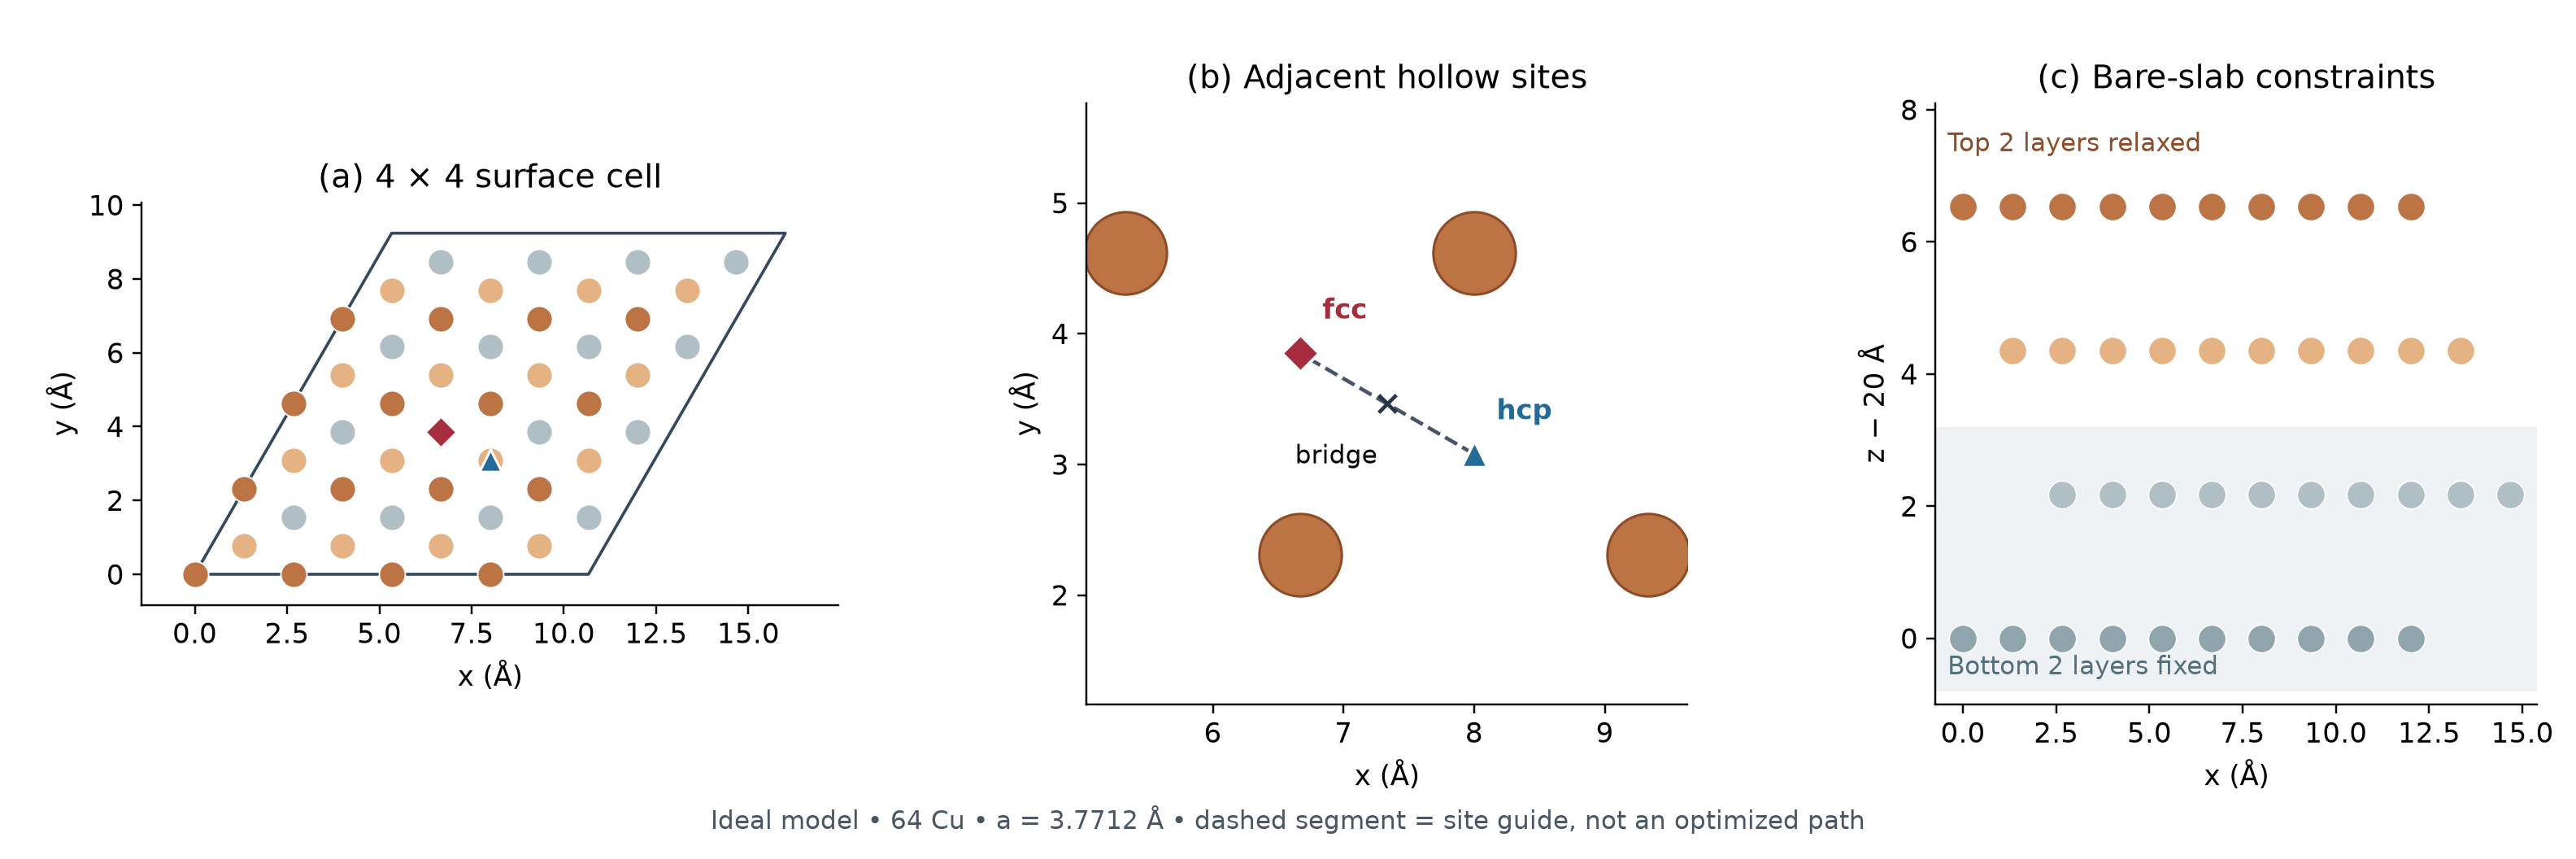
\includegraphics[width=\linewidth]{model-and-sites.png}
\caption{新建理想 Cu(111) 模型及位点定义。左：面内超胞；中：相邻 hcp、fcc 与桥位；
右：裸表面的固定层与放松层。虚线仅连接几何位点，尚非优化后的迁移轨迹。}
\end{figure}
\FloatBarrier

\section{电子结构、反应路径与振动}
\subsection{电子结构和约束驻点}
采用 CP2K 的原生 GFN1-xTB 方法\cite{gfn1,cp2k}，中性、闭壳层电子态。
GFN1-xTB 以参数化紧束缚框架描述电子结构，适于该教学模型的结构、力和路径计算。
固定铜表面时，势能可写为 $E(\mathbf r_{\mathrm O};\mathbf R_{\mathrm{Cu}})$，
驻点条件是氧的三个活动坐标上 $\nabla_{\mathrm O}E=0$。
对固定 Cu 的反作用力并不要求为零。
几何优化不施加空间群保持条件，固定坐标在优化后逐一核对。
自洽场采用 OT-DIIS、\texttt{FULL\_SINGLE\_INVERSE} 预条件器与
\texttt{STRICT} 算法，收敛阈值 $10^{-6}$，内、外迭代上限分别为 20 和 10，不使用电子展宽。
吸附态几何优化的最大与均方根位移阈值分别为 $0.003$、$0.0015\ a_0$，
最大与均方根力阈值分别为 $4.5\times10^{-4}$、$3.0\times10^{-4}\ E_{\mathrm h}/a_0$。
周期超胞共含 710 个显式价电子。

\subsection{NEB 与爬山图像}
以优化后的 hcp 和 fcc 为端点，共设置 5 个图像，其中 3 个为内部图像。
普通 NEB 将真实势能力的垂直分量与沿带切向的弹簧力相加：
\begin{equation}
\mathbf F_i^{\mathrm{NEB}}=-\nabla E_i\big|_\perp+\mathbf F_i^{\mathrm s}\big|_\parallel.
\end{equation}
弹簧维持图像分布，垂直势能力使带靠近最小能量路径。
爬山图像去除弹簧力，并反转势能力的切向分量\cite{cineb}：
\begin{equation}
\mathbf F_i^{\mathrm{CI}}=-\nabla E_i+2(\nabla E_i\cdot\hat{\boldsymbol\tau}_i)\hat{\boldsymbol\tau}_i.
\end{equation}
使用改进切线\cite{tangent}、弹簧常数 $0.05\ E_{\mathrm h}/a_0^2$，不进行图像旋转、平移对齐或端点再优化。
按照课件先做两步普通改进切线 NEB，再启用爬山图像；这是一条逐步收敛的 CI-NEB 路径。
DIIS 带优化上限为 100 步。整带最大与均方根位移阈值为 $0.002$、$0.001\ a_0$，
力阈值为 $0.0045$、$0.003\ E_{\mathrm h}/a_0$\cite{cp2kband}。
路径图以累计氧位移为横坐标，以 hcp 电子能为零点，展示初始带和最终 CI-NEB 离散图像。
路径整体的有效力收敛与峰顶的真实残余梯度分别检验。

\subsection{局域振动与唯一虚频}
使用步长 $0.01\ a_0$ 的有限差分计算 Hessian\cite{cp2kfreq}。
全部铜原子固定时，仅有氧的三个活动自由度，不扣除分子整体平移或转动。
两个吸附极小值应有三个正曲率模式；迁移一阶鞍点应有一个负曲率模式，
其实际位移应沿空穴之间的迁移方向。唯一虚频与小残余梯度共同检验局域鞍点，
再结合连续路径确定其连接的吸附位点。

\section{结构、路径与势垒结果}
\subsection{吸附位点与桥位构型}
裸表面弛豫使最上层平均向内移动约 $0.152\ \text{\AA}$，底部两层保持不变。
在同一铜骨架上，hcp 与 fcc 均形成三配位空穴吸附结构，氧与三个近邻 Cu 的距离分别约为
$1.837$--$1.843$ 和 $1.827$--$1.831\ \text{\AA}$。
fcc 中较短的 O--Cu 距离与其较低的吸附位点能量相一致。
表面弛豫后，三角空穴略偏离理想等边形；根据下层堆垛及三个 Cu 近邻的身份仍可清楚区分 hcp 和 fcc。

\begin{figure}[htbp]
\centering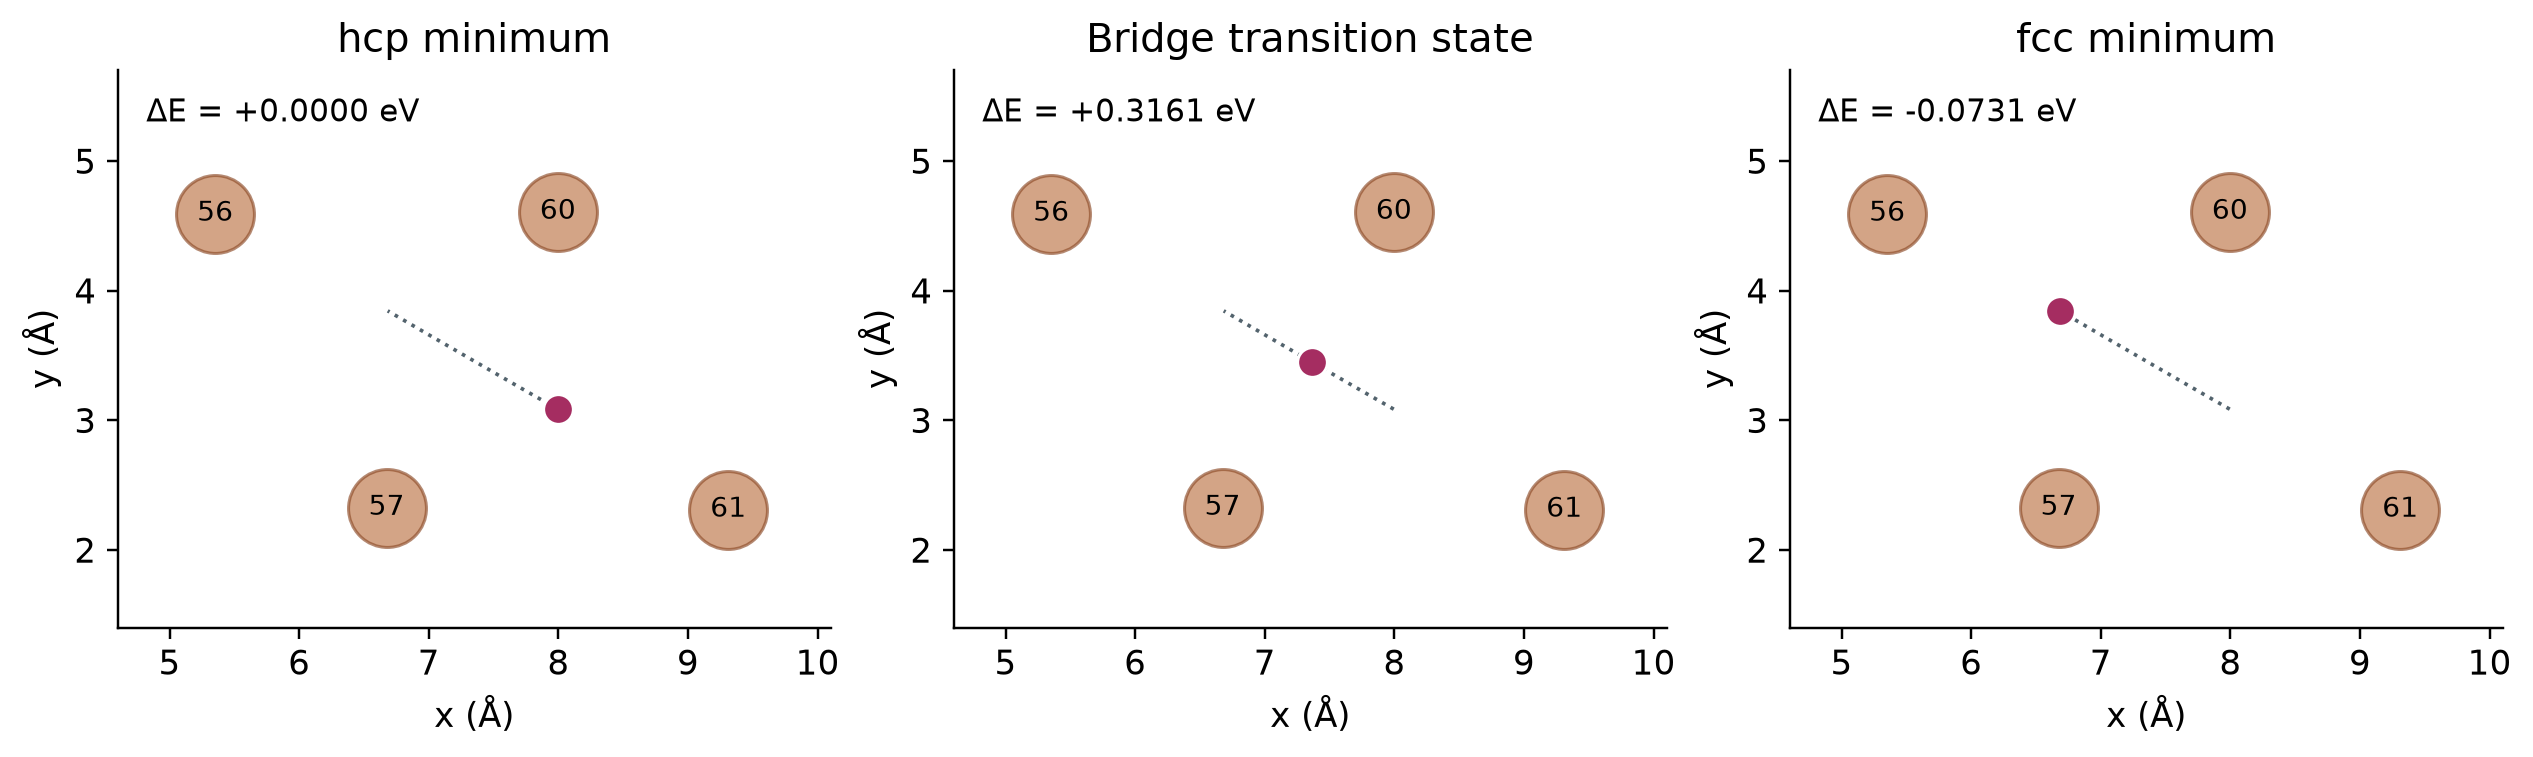
\includegraphics[width=\linewidth]{stationary-structures.png}
\caption{本次计算的 hcp、桥位过渡态和 fcc 构型俯视图。红色为 O，铜色为顶层 Cu。
57、60 为两个空穴共享的顶层 Cu 原子编号；点线为本次计算的五图像路径投影。}
\label{fig:structures}
\end{figure}

过渡态中的 O 主要与共享的 Cu57、Cu60 配位，距离为 $1.7617$、$1.7603\ \text{\AA}$，
第三近邻距离增大到 $2.5395\ \text{\AA}$，因此可识别为桥位构型。
虽然两个 O--Cu 距离缩短，但配位数从三配位降至主要二配位，伴随氧离开较稳定空穴并升高，
总体能量上升。氧的 $z$ 坐标从 hcp 的 $27.4107\ \text{\AA}$ 升至峰顶的
$27.5465\ \text{\AA}$，再降至 fcc 的 $27.3978\ \text{\AA}$。
这体现了迁移时横向运动与表面法向松弛的耦合。

\begin{table}[htbp]
\centering\small
\caption{本次路径中三个特征构型。相对能均以同一最终路径的 hcp 为零点。}
\begin{tabular}{lrrr}
\toprule
构型 & 电子能 / $E_{\mathrm h}$ & 相对电子能 / eV & O 的 $z$ / \AA\\
\midrule
hcp & $-296.663152266927$ & $0.0000$ & 27.4107\\
桥位 TS & $-296.651537547546$ & $0.3161$ & 27.5465\\
fcc & $-296.665837202157$ & $-0.0731$ & 27.3978\\
\bottomrule
\end{tabular}
\end{table}
\FloatBarrier

\subsection{CI-NEB 路径与收敛}
相邻两端的氧位置相距 $1.5153\ \text{\AA}$，最终路径累计长度为 $1.5455\ \text{\AA}$。
三个内部图像相对 hcp 的电子能依次为 $0.1847$、$0.3161$ 和 $0.1576\ \eV$，
第三幅图像是唯一的内部峰。初始直线插值带的峰高约 $0.4454\ \eV$；
允许氧沿法向弛豫后，峰高降至 $0.3161\ \eV$。
因此，用未优化的几何插值直接估计势垒会明显偏高。

\begin{figure}[htbp]
\centering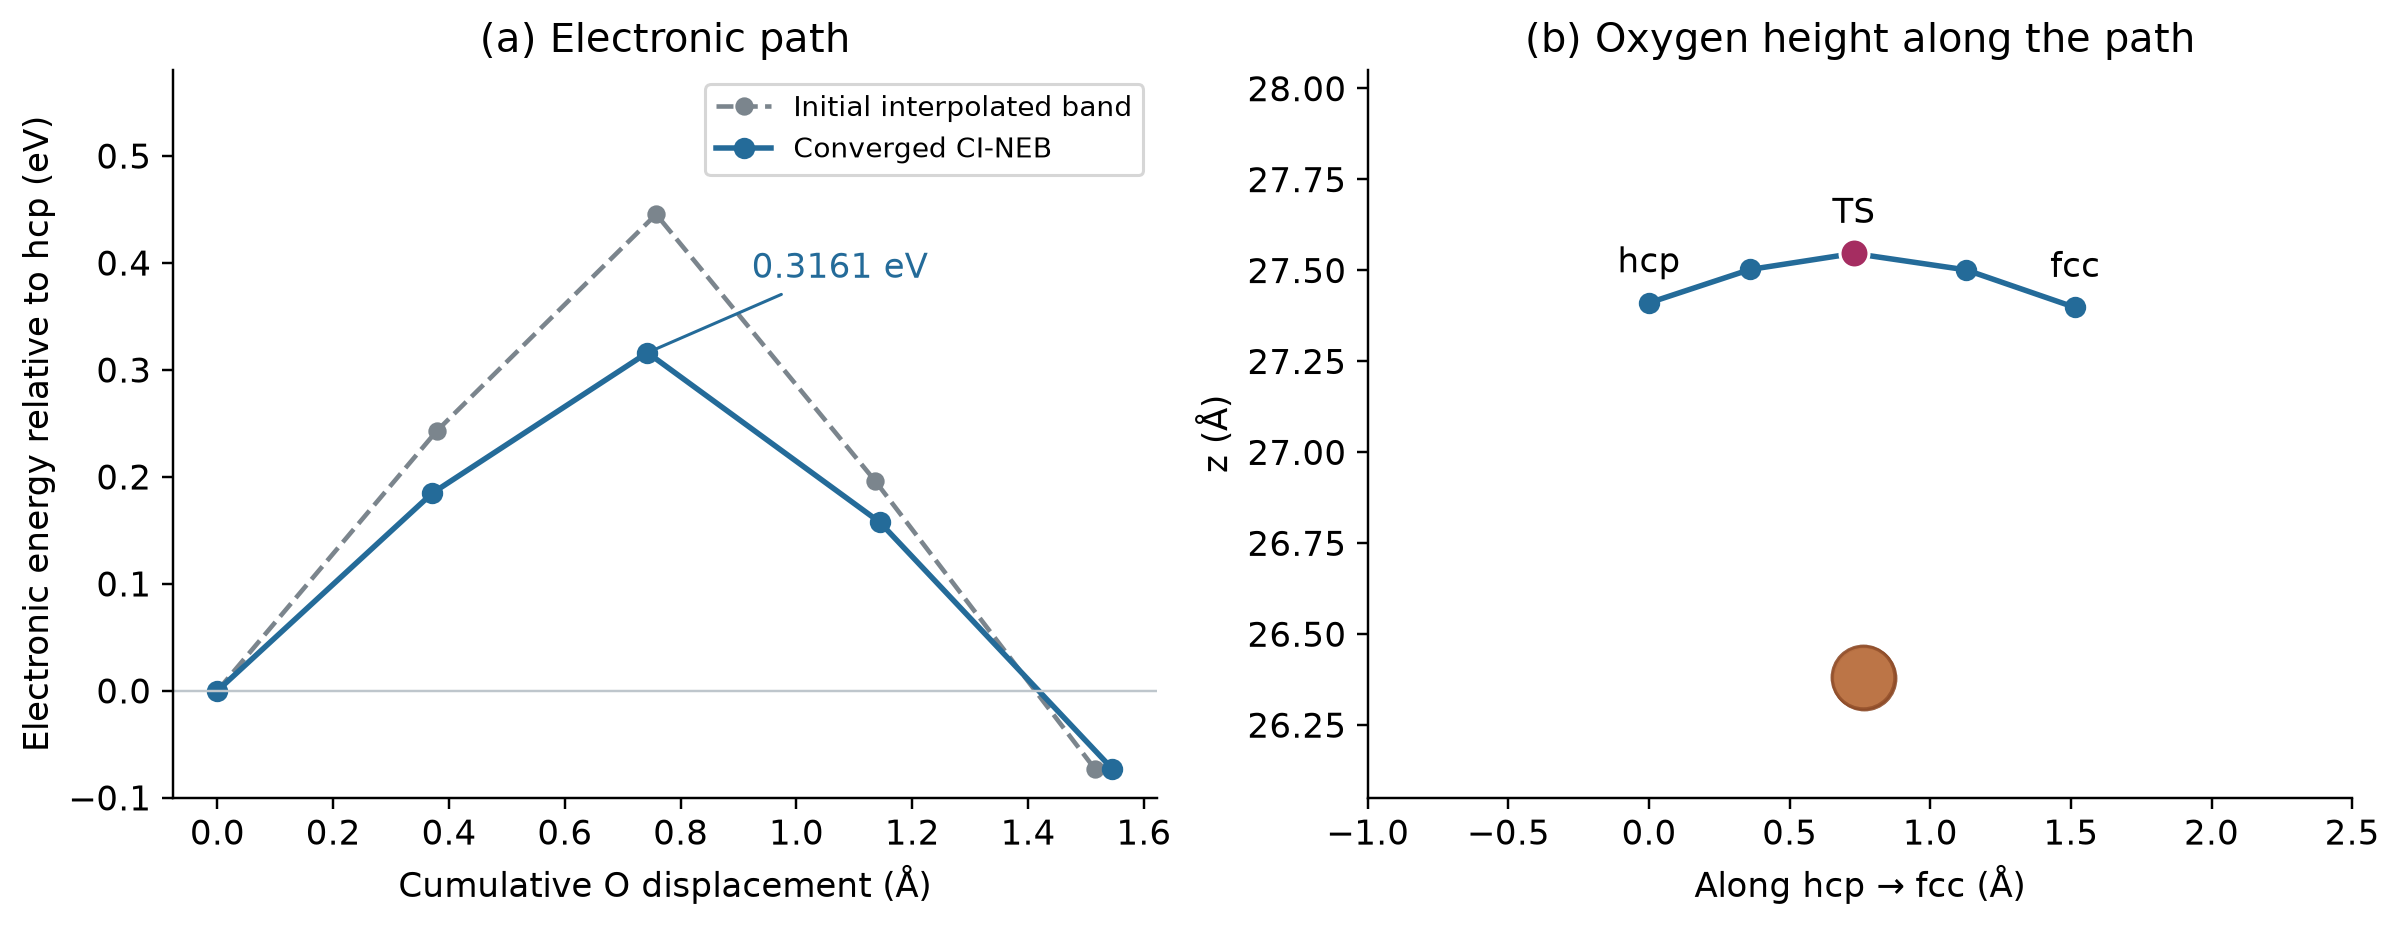
\includegraphics[width=\linewidth]{cineb-path.png}
\caption{左：初始插值带与收敛 CI-NEB 的电子能曲线；连线只连接实际图像。
右：氧沿迁移方向的投影及高度变化。曲线不是 IRC，也不包含逐图像热修正。}
\label{fig:path}
\end{figure}

第 7 步整带四项收敛条件均满足。最终最大有效力为
$7.91\times10^{-5}\ E_{\mathrm h}/a_0$，最大位移为 $1.23\times10^{-4}\ a_0$；
五图像中的全部 Cu 坐标保持不变。
课件的 BAND 力阈值比吸附态优化阈值宽，但本次实际残余有效力已远低于设定阈值。
进一步在峰顶独立计算的真实最大力为 $5.34\times10^{-5}\ E_{\mathrm h}/a_0$
（约 $0.00275\ \eV/\text{\AA}$），表明峰顶已接近活动坐标上的驻点。

\begin{figure}[htbp]
\centering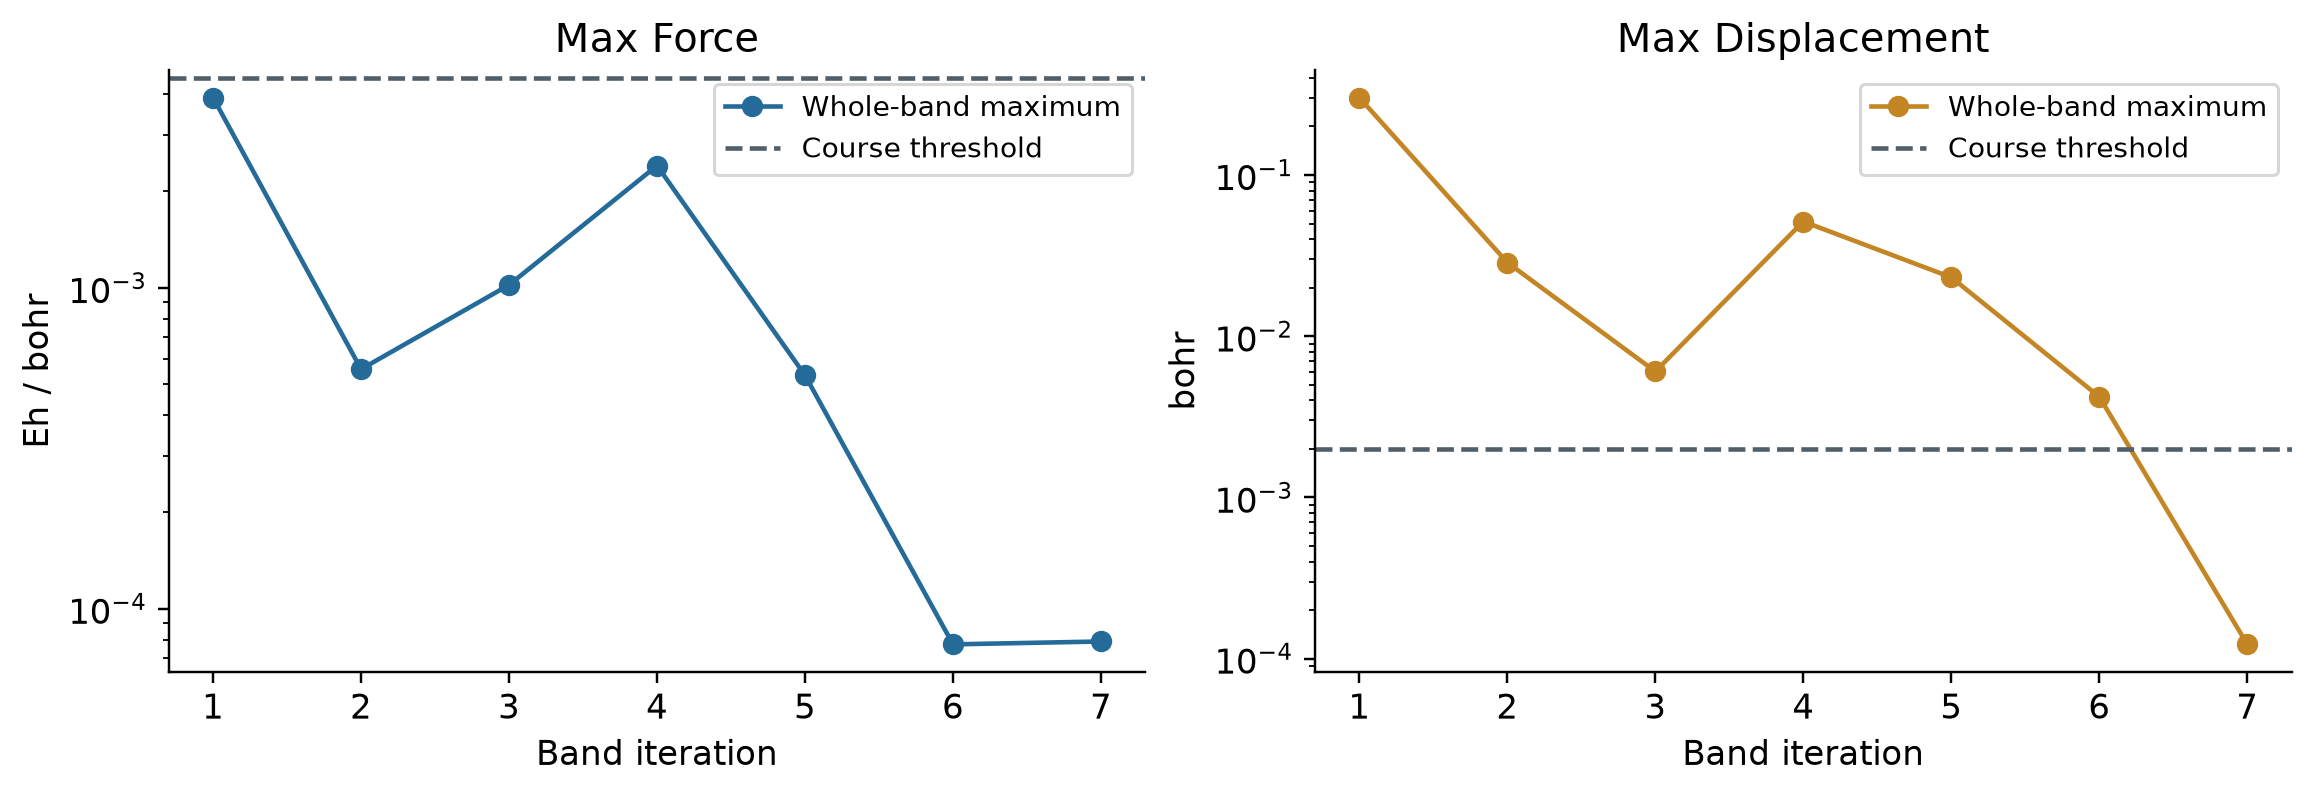
\includegraphics[width=.95\linewidth]{band-convergence.png}
\caption{整带最大有效力和最大位移随迭代的变化，虚线为课件阈值。
优化过程中力与位移可非单调变化，收敛由同一步全部判据共同判断。}
\end{figure}
\FloatBarrier

\subsection{振动核验与迁移模式}
三个特征构型的振动频率见表\ref{tab:freq}。hcp、fcc 的三个活动模式均为实频，
确认二者为固定铜骨架势能面上的极小值。桥位构型只有一个虚频，其氧位移单位方向近似为
$(0.8652,-0.5013,-0.0081)$，与局域路径切向的绝对点积为 $0.99995$。
该模式主要是面内跨桥位迁移；两个稳定模式分别主要对应面内横向运动和表面法向运动。

\begin{table}[htbp]
\centering\caption{氧原子三个活动振动模式，单位为 $\mathrm{cm^{-1}}$。}
\label{tab:freq}
\begin{tabular}{lrrr}
\toprule 构型 & 模式 1 & 模式 2 & 模式 3\\\midrule
hcp & 306.81 & 310.99 & 370.28\\
桥位 TS & $187.29i$ & 418.77 & 444.90\\
fcc & 322.55 & 329.37 & 379.41\\\bottomrule
\end{tabular}
\end{table}

\begin{figure}[htbp]
\centering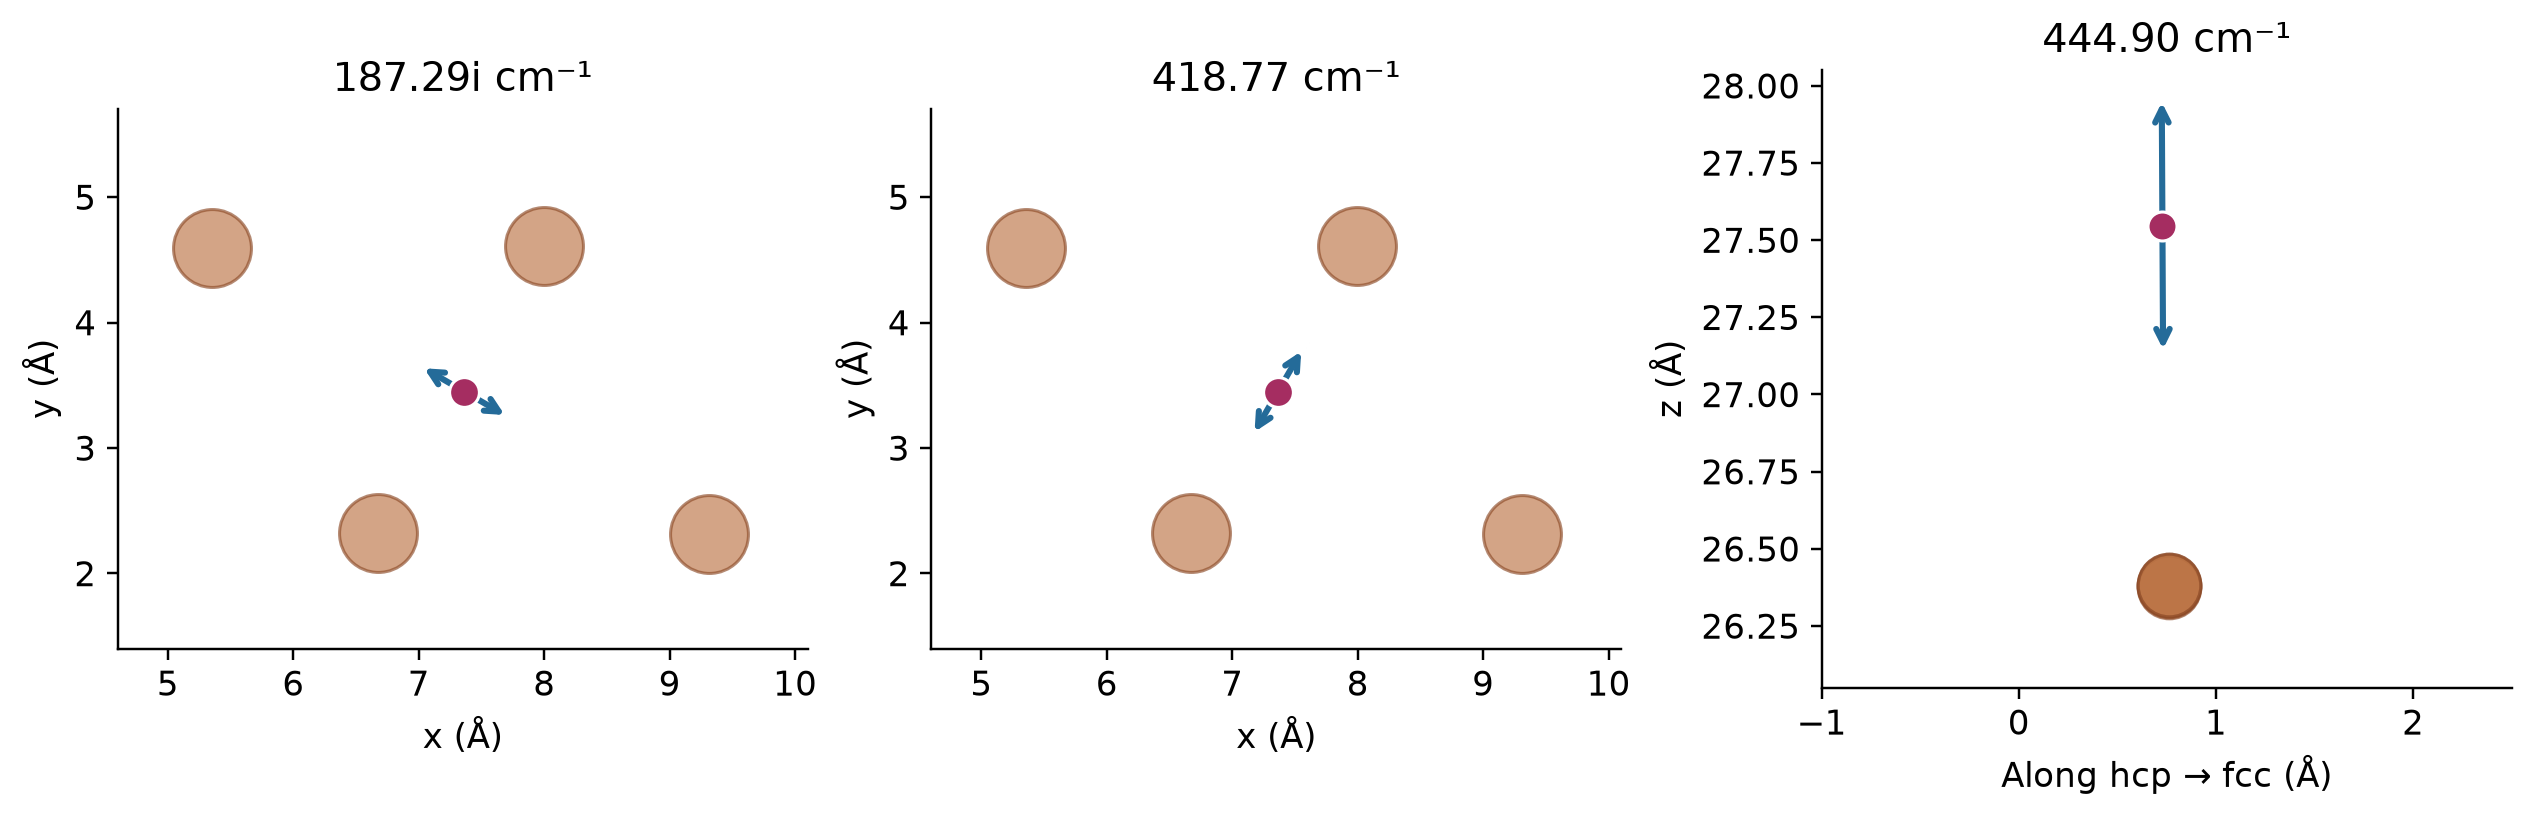
\includegraphics[width=\linewidth]{ts-modes.png}
\caption{桥位三个模式的氧位移方向。前两幅为俯视图，第三幅为侧视图；箭头按统一显示尺度绘制。
虚频方向意味着势能沿该方向下降，而非真实的周期振荡。}
\end{figure}

独立有限差分 Hessian 由氧的六个位移力重建，所得频率与程序输出一致。
对数值 Hessian 的两三角部分及其平均矩阵分别对角化，三个构型的曲率符号均不改变，
频率差均小于 $0.26\ \mathrm{cm^{-1}}$。独立频率计算的基准电子能与路径能量之差
小于 $10^{-5}\ \eV$。这些检验支持当前驻点和曲率判别；未另作步长或模型精度外推。
路径和唯一迁移虚频共同支持 hcp 经桥位连接 fcc 的机理。
\FloatBarrier

\section{能垒与局域谐振动自由能}
电子正向势垒、逆向势垒和位点能差分别定义为
\begin{align}
\Delta E_{\mathrm f}^{\ddagger}&=E_{\mathrm{TS}}-E_{\mathrm{hcp}},\\
\Delta E_{\mathrm r}^{\ddagger}&=E_{\mathrm{TS}}-E_{\mathrm{fcc}},\\
\Delta E&=E_{\mathrm{fcc}}-E_{\mathrm{hcp}}.
\end{align}
三者满足 $\Delta E_{\mathrm f}^{\ddagger}-\Delta E_{\mathrm r}^{\ddagger}=\Delta E$。

在固定晶胞与固定铜表面的局域模型中，以氧的稳定模式计算
\begin{equation}
F_{\mathrm{vib}}(T)=\sum_{j\in\mathrm{stable}}
\left[\frac{h\nu_j}{2}+k_{\mathrm B}T\ln\!\left(1-e^{-h\nu_j/(k_{\mathrm B}T)}\right)\right].
\end{equation}
两个吸附极小值各计入三个实频，鞍点仅计入两个实频，唯一虚频从配分函数中排除。
取 $T=298.15\ \mathrm K$，以 $E+F_{\mathrm{vib}}$ 构造局域谐振动自由能阶梯。
该修正不含铜声子及吸附层的构型熵，也不加入气相分子的平动、转动项。

\begin{table}[htbp]
\centering\small
\caption{298.15 K 下的局域振动热修正，单位为 eV。$F_{\mathrm{loc}}=E+F_{\mathrm{vib}}$。}
\begin{tabular}{lrrrr}
\toprule
构型 & ZPE & $F_{\mathrm{vib}}$ & $\Delta E$ & $\Delta F_{\mathrm{loc}}$\\\midrule
hcp & 0.06125 & 0.04343 & 0.0000 & 0.0000\\
桥位 TS & 0.05354 & 0.04670 & 0.3161 & 0.3193\\
fcc & 0.06393 & 0.04750 & $-0.0731$ & $-0.0690$\\\bottomrule
\end{tabular}
\end{table}

振动修正使正向势垒提高 $0.0033\ \eV$，反向局域自由能垒为 $0.3883\ \eV$，
fcc 相对 hcp 的稳定化减小到 $0.0690\ \eV$。过渡态只计入两个稳定模式，
其零点能比 hcp 低 $0.0077\ \eV$；但 hcp 的三个较低频模式具有更大的振动熵，
在 298.15 K 下使反应物的自由能降低更多，最终使活化自由能略高于电子能垒。

\begin{figure}[htbp]
\centering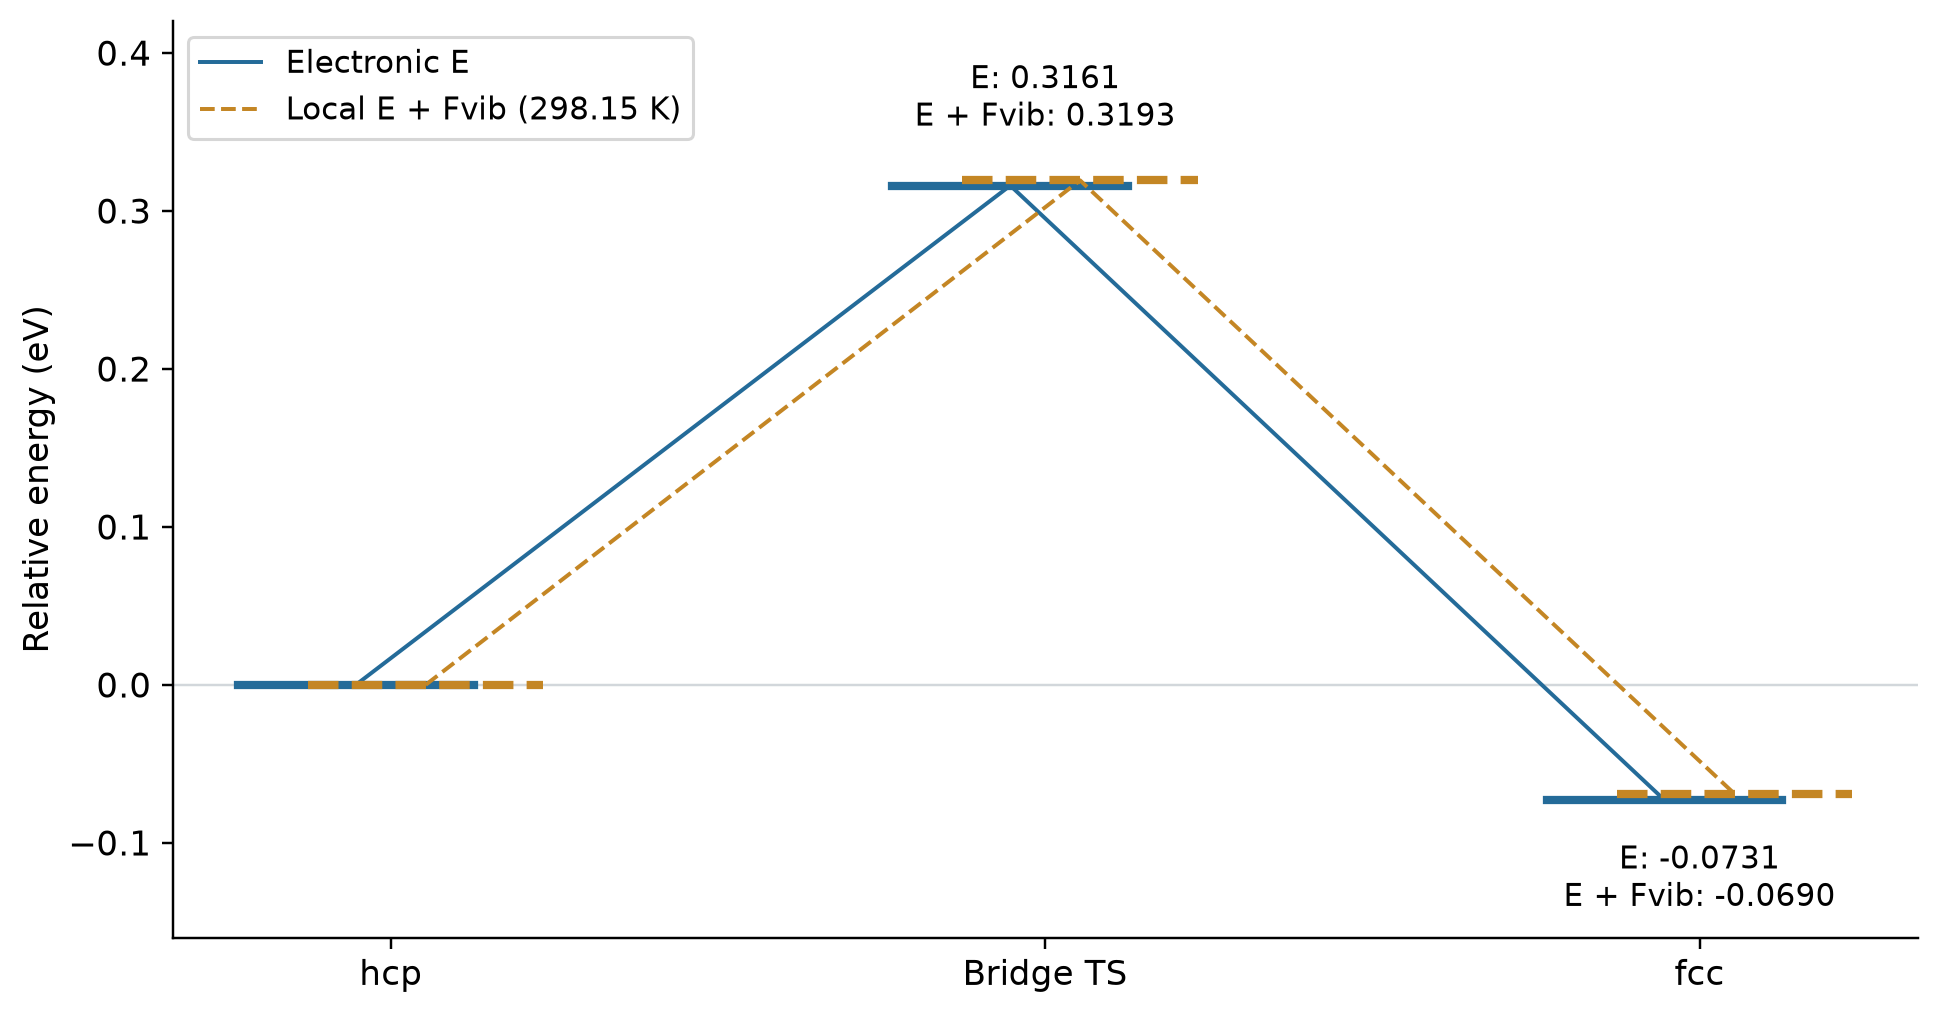
\includegraphics[width=.95\linewidth]{energy-ladder.png}
\caption{电子能与局域谐振动自由能阶梯，均以各自的 hcp 为零点。
该图包含三个离散驻点的热修正，不代表连续自由能路径。}
\label{fig:ladder}
\end{figure}

谐振过渡态理论下，单条跃迁通道的速率为
\begin{equation}
k(T)=\frac{k_{\mathrm B}T}{h}\exp\!\left[-\frac{\Delta F_{\mathrm{loc}}^{\ddagger}}{k_{\mathrm B}T}\right].
\end{equation}
这一表达式采用反应物盆地内热平衡、局域谐振及穿过分界面后不再返回的近似，
不计隧穿，且未乘等价出口数；它是单跃迁速率而非表面扩散系数。
代入本次 $\Delta F_{\mathrm{loc}}^{\ddagger}=0.3193\ \eV$，得到
$k_{\mathrm{hcp}\to\mathrm{fcc}}(298.15\ \mathrm K)\approx2.49\times10^7\ \mathrm{s^{-1}}$。
这是固定铜骨架上的单通道谐振过渡态估计。实际扩散还取决于等价出口、反向跃迁、
吸附覆盖度、铜表面振动及可能的再穿越，不能仅凭这一速率确定宏观扩散系数。
\FloatBarrier

\section{课件对照与方法讨论}
课件第 26 页的能量表给出 hcp、TS、fcc 分别为
$-296.664375$、$-296.651725$、$-296.666948\ E_{\mathrm h}$\cite{course}。
按表中数值换算，正向峰高为 $0.3442\ \eV$，fcc 相对 hcp 为 $-0.0700\ \eV$。
本次对应为 $0.3161$ 和 $-0.0731\ \eV$：位点稳定性次序相同，位点能差仅相差约
$0.0030\ \eV$，峰高低约 $0.0282\ \eV$。

\begin{table}[htbp]
\centering
\caption{本次结果与课件示例的电子能差对照，单位为 eV。}
\begin{tabular}{lrr}
\toprule 物理量 & 本次计算 & 课件表格换算\\\midrule
hcp $\to$ TS & 0.3161 & 0.3442\\
fcc $\to$ TS & 0.3891 & 0.4142\\
hcp $\to$ fcc & $-0.0731$ & $-0.0700$\\\bottomrule
\end{tabular}
\end{table}

课件页标题虽使用 Gibbs 自由能表述，但图轴标为 $E/\eV$，所示表格未列振动热校正；
因此这里将其表值与本次电子能差对照，而将本次独立得到的局域振动自由能另列。
本次保持底层坐标严格固定，所得表面弛豫构型与课件示例并非已证明完全相同。
势垒差反映具体表面结构和数值实现的综合差别，不能仅凭这组对照归因于某一因素。

课件的 GFN1-xTB、OT-DIIS 和 $10^{-6}$ SCF 阈值在本模型中能够收敛。
裸表面保留空间群会使名义固定底层发生约 $0.097\ \text{\AA}$ 的投影位移；
关闭空间群保持后可同时满足电子、几何收敛和固定层要求。
这说明电子迭代收敛与几何约束正确性是不同的检查：必须以最终坐标验证所研究的表面模型。

GFN1-xTB 是参数化的紧束缚近似\cite{gfn1}，本次结论对应低覆盖度、固定铜骨架上的单氧迁移。
五图像带和三活动坐标频率足以刻画本次相邻空穴间的局域通道；若研究表面重构、
更高覆盖度或定量扩散系数，则需扩大活动原子集合并检验超胞、图像数及电子结构方法的影响。

\section{结论}
Cu(111) 表面氧从 hcp 三重空穴经桥位迁移至相邻 fcc 三重空穴。
fcc 比 hcp 稳定 $0.0731\ \eV$；正、逆电子能垒为 $0.3161$ 和 $0.3891\ \eV$。
桥位具有唯一的 $187.29i\ \mathrm{cm^{-1}}$ 面内迁移模式，与五图像路径的切向一致。
在 $298.15\ \mathrm K$ 下，局域谐振动修正后的正、逆势垒为 $0.3193$ 和 $0.3883\ \eV$，
不改变 fcc 更稳定的结论。与课件示例相比，稳定性次序和能量尺度一致。

配套结果含三个驻点的 CIF、五图像 XYZ/PDB、迁移动画及虚频模式动画。
迁移动画在五个实际图像间作几何插值，虚频动画按计算本征向量展示失稳方向。

\section*{数据与代码}
本实验的计算输入、关键输出、结构与频率数据、后处理脚本、图表动画和报告源文件
公开于 \url{https://github.com/populuscathayana/Quantum5}。
仓库提供离线结果核验与报告重建说明，电子能和局域振动自由能分别保存。

\begin{thebibliography}{9}
\bibitem{course} 浙江大学量子化学实验课件. CuO：Cu(111) 表面氧原子迁移.
\bibitem{gfn1} Grimme S, Bannwarth C, Shushkov P. A robust and accurate tight-binding quantum chemical method
for structures, vibrational frequencies, and noncovalent interactions of large molecular systems
parametrized for all spd-block elements ($Z=1$--86). \textit{J. Chem. Theory Comput.}, 2017, 13: 1989--2009.
\href{https://doi.org/10.1021/acs.jctc.7b00118}{doi:10.1021/acs.jctc.7b00118}.
\bibitem{cp2k} CP2K 2026.2. Native xTB input reference.
\url{https://manual.cp2k.org/cp2k-2026_2-branch/CP2K_INPUT/FORCE_EVAL/DFT/QS/XTB.html}.
\bibitem{cineb} Henkelman G, Uberuaga B P, Jónsson H. A climbing image nudged elastic band method for
finding saddle points and minimum energy paths. \textit{J. Chem. Phys.}, 2000, 113: 9901--9904.
\href{https://doi.org/10.1063/1.1329672}{doi:10.1063/1.1329672}.
\bibitem{cp2kfreq} CP2K 2026.2. Vibrational analysis input reference.
\url{https://manual.cp2k.org/cp2k-2026_2-branch/CP2K_INPUT/VIBRATIONAL_ANALYSIS.html}.
\bibitem{tangent} Henkelman G, Jónsson H. Improved tangent estimate in the nudged elastic band method for finding
minimum energy paths and saddle points. \textit{J. Chem. Phys.}, 2000, 113: 9978--9985.
\href{https://doi.org/10.1063/1.1323224}{doi:10.1063/1.1323224}.
\bibitem{cp2kband} CP2K 2026.2. Band input reference.
\url{https://manual.cp2k.org/cp2k-2026_2-branch/CP2K_INPUT/MOTION/BAND.html}.
\end{thebibliography}
\end{document}
